\documentclass[]{article}
\usepackage[top=2.5cm, bottom=2.5cm, left=3cm, right=3cm]{geometry}
\usepackage{amsmath,amssymb,amsfonts,latexsym,textcomp} %paquetes matematicos
\usepackage{array,multirow,multicol,booktabs,tabulary} %tablas y arrays
\usepackage{graphicx}   
\usepackage{caption,float,subfigure} %float=figuras flotantes.
\usepackage{verbatim}  %texto raw 
\usepackage[ampersand]{easylist} %http://en.wikibooks.org/wiki/LaTeX/List_Structures#Easylist_package 
\usepackage{subfigure}
\usepackage{color}
\usepackage[usenames,dvipsnames,svgnames,table,x11names]{xcolor} 

%---- Usar otros fonts + símbolo \degree -----------------------------------
\newcommand*{\myfont}{\fontfamily{lmtt}\selectfont}
\DeclareTextFontCommand{\textmyfont}{\myfont}	
\usepackage{gensymb} 

%---- Code highlighting con Listings ---------------------------------------
\usepackage{listings}	
\definecolor{mygreen}{rgb}{0.5,0.6,0.5}
\definecolor{mygray}{rgb}{0.5,0.5,0.5}
\definecolor{mymauve}{rgb}{0.58,0,0.82}
\definecolor{mygray2}{rgb}{0.9764, 0.9764, 0.9762}
%---- Config listings ------------------------------------------------------
\lstset{ %
	backgroundcolor=\color{mygray2},	% background color
	basicstyle=\footnotesize\ttfamily,	% tamaño de las letras y tipo de letra
	breaklines=true,	% corte de linea (line breaking)solo en espacio blanco
	captionpos=t,		% posicion del caption b,t,n (top,bottom,none)
	commentstyle=\color{ForestGreen},	% estilo del comentario
	%escapeinside={\%*}{*},	% si se desea agregar codigo Latex dentro el codigo debe ser %*codigo latex*
	frame=single,	% agrega marco al codigo
	frameround=tttt,	% redondear el marco
	keepspaces=true,	% mantiene los espacios en el texto, util para mantener la indentacion del codigo (uso posible en columns=flexible)
	keywordstyle=\color{blue},	% estilo de los keywords
	stringstyle=\color{mymauve},	% estilo del string
	numbers=left,	% donde poner los numeros de linea, (none, left, right)
	numbersep=5pt,	% cuan lejos los numeros de linea estan del codigo
	xleftmargin=0pt,	% margen izquierdo
	showspaces=false,	% muestra espacios de codigo en todas partes usando el caracter barra baja "_", sobreescribe el comando 'showstringspaces'
	showstringspaces=false,	% muestra espacios solo en los strings
	tabsize=2,	% tabulacion por defecto =2
	title=\lstname	% muestra el nombre de lo archivos incluidos con \lstinputlisting; tambien se puede tratar con caption en vez de title
}	
%---- Config personalizada del caption -------------------------------------
\DeclareCaptionFont{white}{ \color{white} }
\DeclareCaptionFormat{listing}{
	\colorbox[cmyk]{0.43, 0.35, 0.35, 0.01 }{
		\parbox{0.96\linewidth}{\hspace{15pt}#1#2#3}
	}
}
\captionsetup[lstlisting]{ format=listing, 
	labelfont=white, 
	textfont=white, 
	singlelinecheck=false, 
	margin=0pt, 
	font={bf,footnotesize} }
%---- Caracteres especiales ------------------------------------------------	
% Por defecto, listings no soporta inputec para mostrar los acentos y caracteres especiales.
% para manejar utf8 se debe enlistar los caracteres segun:
\lstset{literate=
	{á}{{\'a}}1 {é}{{\'e}}1 {í}{{\'i}}1 {ó}{{\'o}}1 {ú}{{\'u}}1
	{Á}{{\'A}}1 {É}{{\'E}}1 {Í}{{\'I}}1 {Ó}{{\'O}}1 {Ú}{{\'U}}1
	{à}{{\`a}}1 {è}{{\`e}}1 {ì}{{\`i}}1 {ò}{{\`o}}1 {ù}{{\`u}}1
	{À}{{\`A}}1 {È}{{\'E}}1 {Ì}{{\`I}}1 {Ò}{{\`O}}1 {Ù}{{\`U}}1
	{ä}{{\"a}}1 {ë}{{\"e}}1 {ï}{{\"i}}1 {ö}{{\"o}}1 {ü}{{\"u}}1
	{Ä}{{\"A}}1 {Ë}{{\"E}}1 {Ï}{{\"I}}1 {Ö}{{\"O}}1 {Ü}{{\"U}}1
	{â}{{\^a}}1 {ê}{{\^e}}1 {î}{{\^i}}1 {ô}{{\^o}}1 {û}{{\^u}}1
	{Â}{{\^A}}1 {Ê}{{\^E}}1 {Î}{{\^I}}1 {Ô}{{\^O}}1 {Û}{{\^U}}1
	{œ}{{\oe}}1 {Œ}{{\OE}}1 {æ}{{\ae}}1 {Æ}{{\AE}}1 {ß}{{\ss}}1
	{ç}{{\c c}}1 {Ç}{{\c C}}1 {ø}{{\o}}1 {å}{{\r a}}1 {Å}{{\r A}}1
	{ñ}{{\~n}}1 {£}{{\pounds}}1 {°}{{\degree}}1
}		
%---- Macro de inclusión de documentos con listings ------------------------
% [2]=numero de argumentos, #1=argumento 1, #2=argumento 2
\newcommand{\includecode}[2]{\lstinputlisting[language=#1, caption=#2, label=#2]{#2}}			

% --- Fig and table command -----------------------------------------------
%\newcommand{\figref}[1]{\figurename~\ref{#1}}
\newcommand{\figref}[1]{Fig.~\ref{#1}}
\newcommand{\tabref}[1]{Table~\ref{#1}}
\newcommand{\algref}[1]{Algorithm~\ref{#1}}


%=============================================================================================
%opening
\title{EE4323 Industrial Control Systems\\ 
		Homework Assignment 2\\
		\underline{Nonlinear DC moto}r}
\author{Paulo R. Loma Marconi}
\date{June 13, 2017}

\begin{document}
\maketitle

\section{Introduction}
The objective is to simulate a nonlinear electro-mechanical system with thermal model and static Coulomb friction. We use three ODE solvers, the embedded Matlab solver \texttt{ode45}, and two external solvers, the 4th and 5th order Runge-Kutta algorithm \texttt{ode45m}, and the basic Euler algorithm \texttt{eufix1}.

\section{Nonlinear model}
The dynamics of the DC motor has two nonlinear parameters is, 
\begin{align}
	R_A i_A + L_A \dot{i}_A+\alpha \omega_1                             & = e_{i}(t)   \\
	J_1 \dot{\omega}_1 + B_1 \omega_1 - r_1 f_c                         & = \alpha i_A \\
	J_2 \dot{\omega}_2 + B_2 \omega_2 + B_{2C}~sign(\omega_2) + r_2 f_c & = -\tau_{L}  \\
	C_{TM} \dot{\theta}_M + \frac{(\theta_M-\theta_A)}{R_{TM}}          & = i^2_A R_A
\end{align}
where $R_A$ is the stationary resistance, $L_A$ is the stationary inductance, $i_A$ is the input stationary current, $\alpha$ is the internal parameters, $\omega$ is the angular speed, $e_i(t)$ is the applied armature voltage, $B$ is the rotational viscous-damping coefficient, $J$ is the moment of inertia, $f_c$ is the contact force between two gears, $r$ is the gear radius, and $B_{2C}$ is the static Coulomb friction. The thermal model is similar to an electrical capacitor-resistor model with thermal capacity $C_{TM}$, $R_{TM}$ is the resistive losses to ambient temperature, $\theta_M$ is the motor temperature, and $\theta_A$ is the ambient temperature. 

Now let us define the sate-vector differential equations: state vector $x = [ i_A~ \omega_2~ \theta_M ]^T $, and input vector $u = [ e_{i}~ \tau_{L}~ \theta_A ]^T$. 

For $\omega_1=N \omega_2$ and $N=\frac{r_2}{r_1}$, eliminating $f_c$ we have

\begin{align}
	\dot{i}_A      & = -\frac{R_A}{L_A}\ i_A - \frac{N \alpha}{L_A} \omega_2 + \frac{1}{L_A} e_{i}                         \\
	\dot{\omega}_2 & = \frac{N \alpha}{J_{eq}} i_A - \frac{B_{eq}}{J_{eq}} \omega_2 - \frac{B_{2C}}{J_{eq}} sign(\omega_2) - \frac{1}{J_eq}\tau_{L} \\
	\dot{\theta}_M & = \frac{R_A}{C_{TM}} i^2_A - \frac{1}{C_{TM} R_{TM}} \theta_M + \frac{1}{C_{TM} R_{TM}} \theta_A
\end{align}
where $J_{eq}=J_2+N^2 J_1$ and $B_{eq}=B_2+N^2 B_1$. 

For simulation purpose only we can simplify as 
\begin{align}
	\dot{i}_A      & = -a~ i_A - b~ \omega_2 + \frac{1}{L_A}e_{i}                        \\
	\dot{\omega}_2 & = c~ i_A - d~ \omega_2 - e~ sign(\omega_2) - \frac{1}{J_eq}\tau_{L} \\
	\dot{\theta}_M & = f~ i^2_A - g~ \theta_M + g~ \theta_A
\end{align}
where $a=\frac{R_A}{L_A}$, $b=\frac{N \alpha}{L_A}$, $c=\frac{N \alpha}{J_{eq}}$, $d=\frac{B_{eq}}{J_{eq}}$, $e=\frac{B_{2C}}{J_{eq}}$, $f=\frac{R_A}{C_{TM}}$, and $g=\frac{1}{C_{TM} R_{TM}}$.



\section{Matlab Scripts}

\subsection{ODE solver \texttt{ode45m}}
\lstinputlisting[language=matlab,caption={ode45m},label={cod:}]{../Matlab/ode45m.m}

\subsection{ODE solver \texttt{eufix1}}
\lstinputlisting[language=matlab,caption={eufix1},label={cod:}]{../Matlab/eufix1.m}

\subsection{Nonlinear model}
In line 37 and 38, the input $e_i$ can be changed from constant input to sinusoidal input.
\lstinputlisting[language=matlab,caption={Nonlinear model},label={cod:}]{../Matlab/asst02_2017.m}

\subsection{Main}
Change the input values in line 5-8, the \verb|input_type| $E_0$ to constant or sinusoidal, and the step size in line 9. 

\textbf{Note:} This script is an example only. In the \textbf{Simulation Results} section we will analyze different scenarios.

\lstinputlisting[language=tex,caption={Main},label={cod:}]{../Matlab/run_asst02_2017.m}

\section{Simulation scenarios}
Two types of scenarios are simulated, \tabref{tab:Sce_1-2}. The first one is submitted to a constant input, low stiction, and two step sizes. The second scenario is more interesting because we study the behaviour due to a sinusoidal input which emulates the reversing mode of the motor at $5[Hz]$ with higher stiction. Both scenarios have load torque at $t=0.2[s]$.

\begin{table}[!ht]
	\centering
	\scalebox{1}{
		\begin{tabular}{c|l|l|l|l}
			&     \multicolumn{2}{c|}{\bf{Scenario 1}}      &       \multicolumn{2}{c}{\bf{Scenario 2}}       \\
			\hline
			\texttt{ode45m} step size & $1\times 10^{-3}$ & $1\times 10^{-4}$         & \multicolumn{2}{l}{$1\times 10^{-4}$}           \\
			\hline
			\texttt{eufix1} step size & $1\times 10^{-3}$ & $1\times 10^{-4}$         & \multicolumn{2}{l}{$1\times 10^{-4}$}           \\
			\hline
			\texttt{ode45} step size  & \multicolumn{2}{l|}{auto}                     & \multicolumn{2}{l}{auto}                        \\
			\hline
			$e_i$           & \multicolumn{2}{l|}{$E_0$}                    & \multicolumn{2}{l}{$E_0 \sin[5(2\pi)(t-0.05)]$} \\
			\hline
			$E_0$           & \multicolumn{2}{l|}{$120~[V]$}                & \multicolumn{2}{l}{$120~[V]$}                   \\
			\hline
			$\tau_{L}$         & \multicolumn{2}{l|}{$80~[N m]$ at $t=0.2[s]$} & \multicolumn{2}{l}{$80~[N m]$ at $t=0.2[s]$}    \\
			\hline
			$\theta_A$         & \multicolumn{2}{l|}{$18~[\degree C]$}         & \multicolumn{2}{l}{$18~[\degree C]$}            \\
			\hline
			$B_{2C}$          & \multicolumn{2}{l|}{$80~[N]$}                 & \multicolumn{2}{l}{$300~[N]$}
		\end{tabular} 		
	}
	\caption{Scenario 1 and 2.}
	\label{tab:Sce_1-2}
\end{table}

\section{Simulation Results}
\subsection*{Scenario 1}
The result in \figref{fig:Sce1} shows the output states due to constant input $E_0=120$, and $B_{2C}=80$. The current overshoot at $0.05[s]$ is due to the inertia that the motor has to overcome. After the inertia is broken, the current $i_A$ drops down to a constant value. The load torque $\tau_{L}$ is applied at $0.2[s]$ which produces the increment in the current and the decrement in the angular velocity. Also, \texttt{eufix1} solves the system with noticeable error, this result is analyzed later. 

\begin{figure}[H]
	\centering
	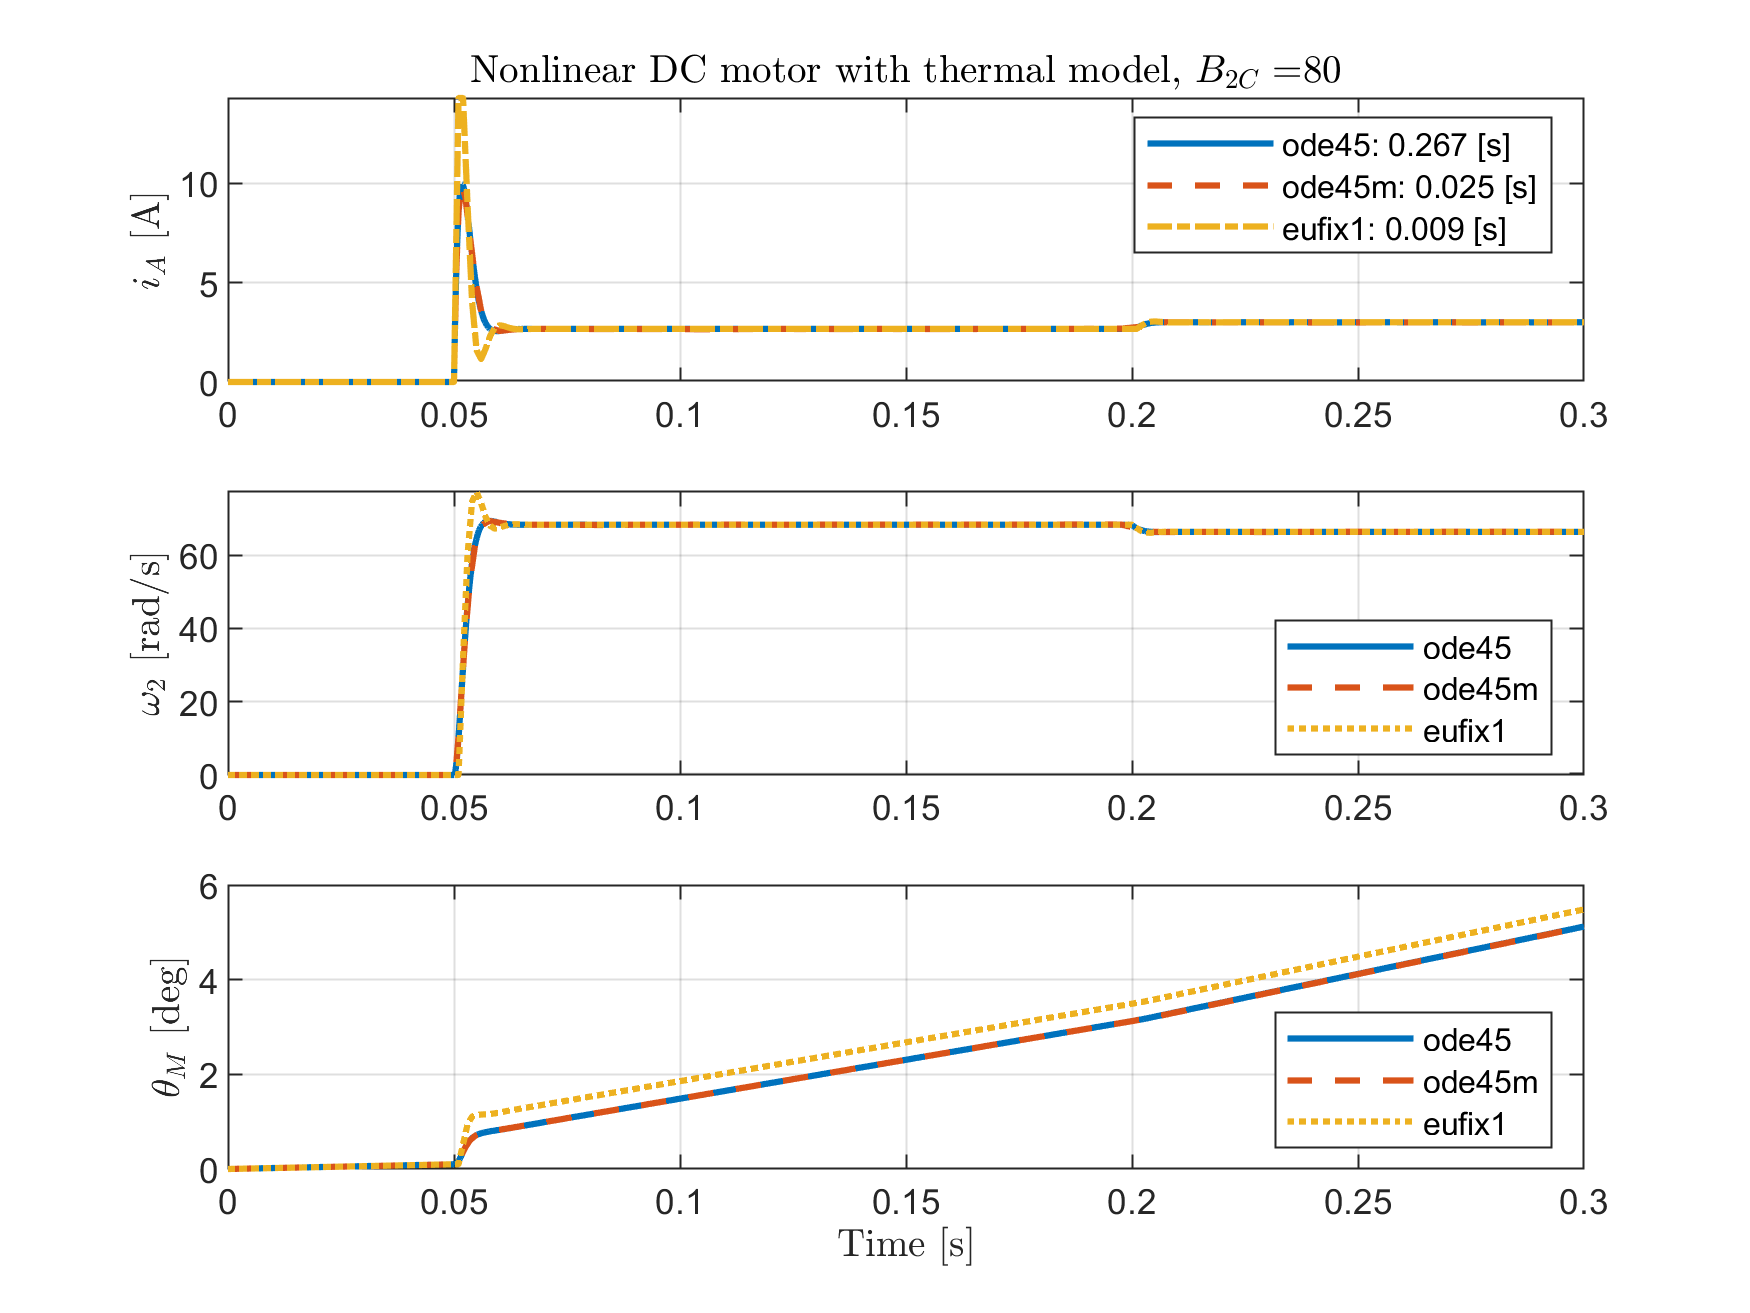
\includegraphics[width=1\linewidth]{E0_ode45-ode45m-eufix1_1e-3}
	\caption{Scenario 1: step size $1\times 10^{-3}$}
	\label{fig:Sce1}
\end{figure}

The time simulation of each solver indicates that \texttt{ode45} is 10 times slower than \texttt{ode45m} and 30 times slower than \texttt{eufix1}. 
\begin{table}[!ht]
	\centering
	\scalebox{1}{
		\begin{tabular}{c|c|c|c}
			                     & \bf{ode45} & \bf{ode45m} & \bf{eufix1} \\
			\hline
			  simulation time [s]   & $0.267$ & $0.025$  & $0.009$  \\
			\hline
			number of time steps &  $71769$   &   $15133$   &   $80001$
		\end{tabular} 		
	}
	\caption{Scenario 1: simulation time and number of steps.}
	\label{tab:}
\end{table}

The temperature of the motor $\theta_M$ increases linearly and reaches steady-state at $45[s]$ approximately, which indicates that the motor won't reach unsafe temperatures.
\begin{figure}[H]
	\centering
	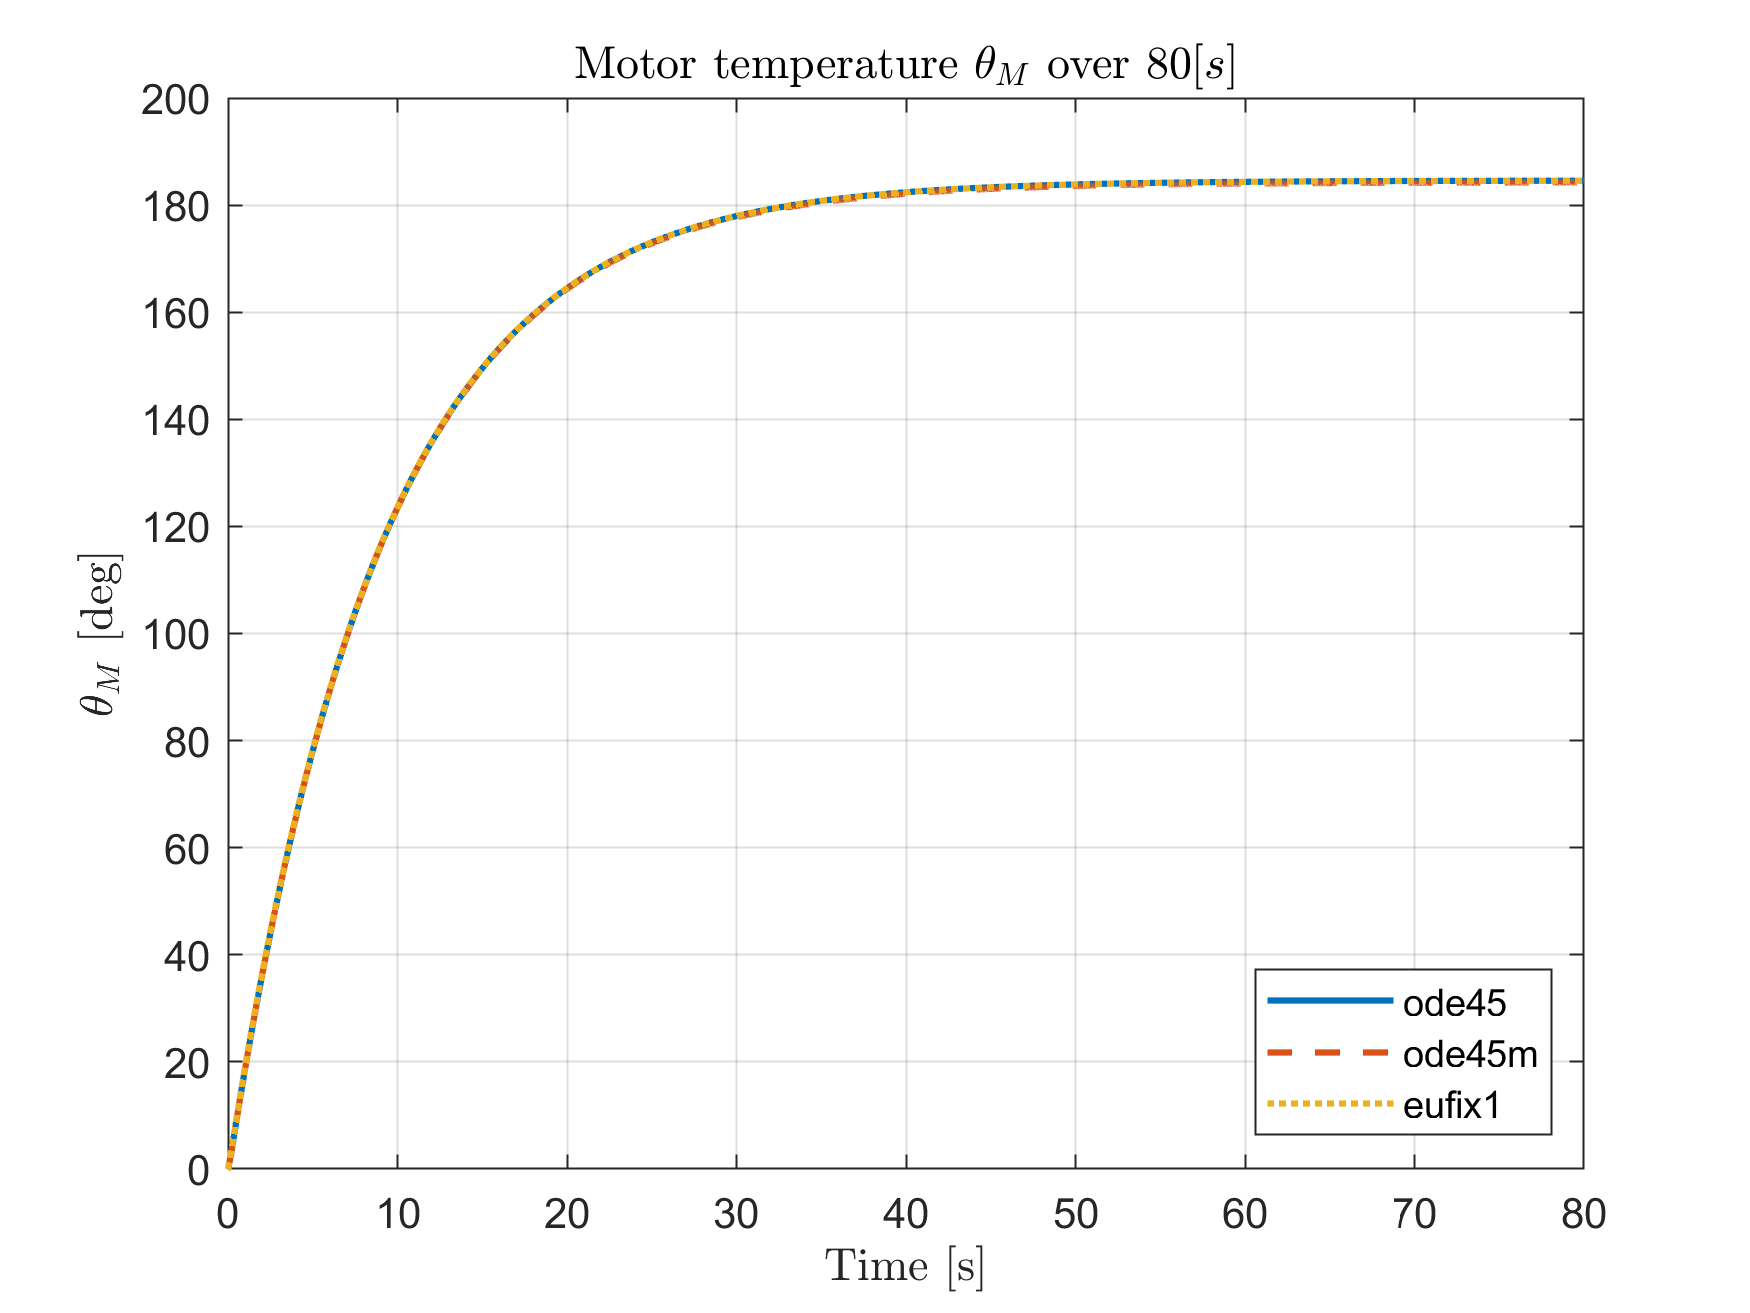
\includegraphics[width=0.65\linewidth]{thetaM_ode45-ode45m-eufix1_1e-3}
	\caption{Scenario 1: $\theta_M$ over $80[s]$}
	\label{fig:Sce1_thetaM}
\end{figure}

Although, \texttt{eufix1} is the fastest solver, with step size of $1\times 10^{-3}$, \texttt{eufix1} outputs the worst performance. The result can be improved if the steps size is decreased to $1\times 10^{-4}$. \figref{fig:Sce1_zoom_a} and \figref{fig:Sce1_zoom_b} show the relative error at max current and max angular velocity between \texttt{ode45} and \texttt{eufix1}.

\begin{figure}[H]
	\centering
	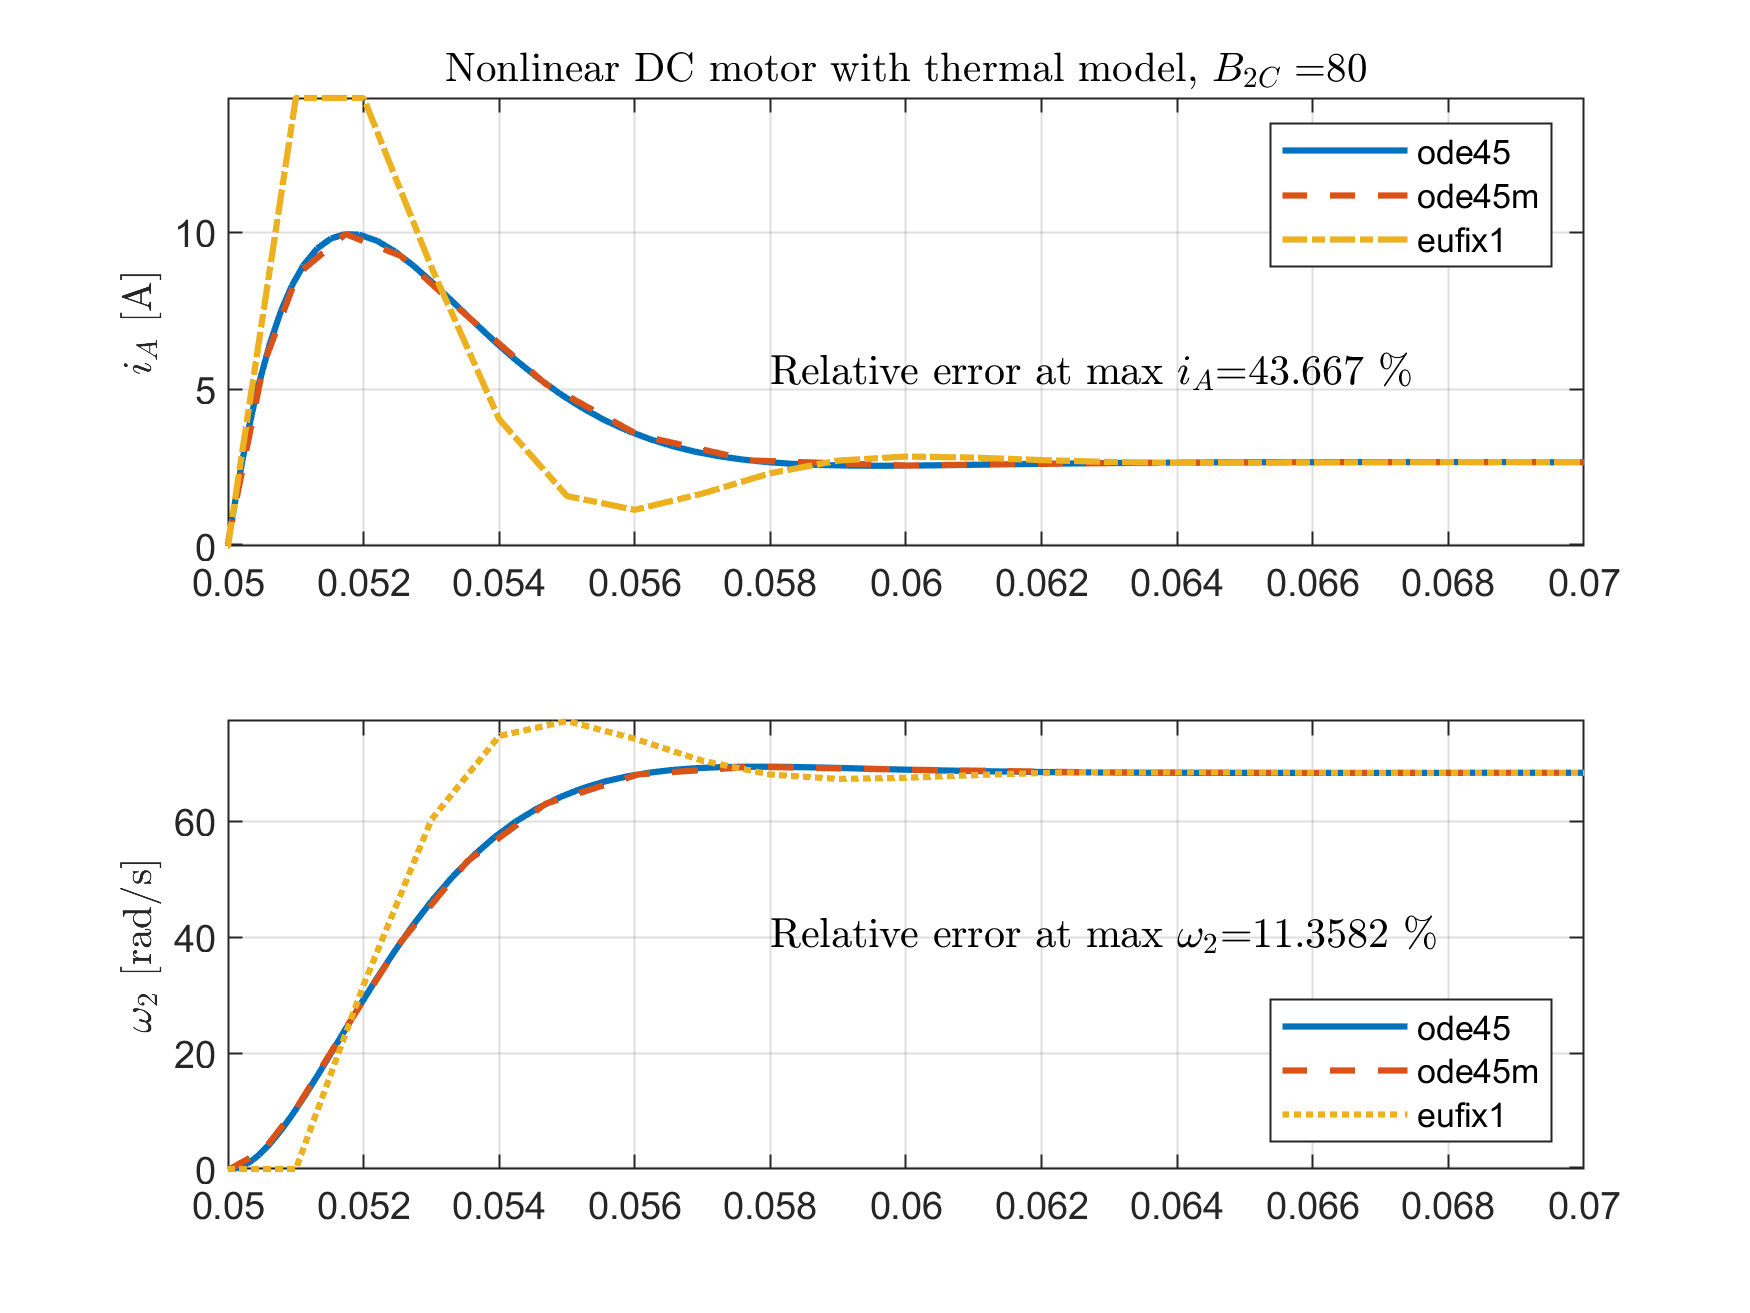
\includegraphics[width=0.80\linewidth]{E0_ode45-ode45m-eufix1_1e-3_zoom}
	\caption{Scenario 1: step size $1\times 10^{-3}$}
	\label{fig:Sce1_zoom_a}
\end{figure}

\begin{figure}[H]
	\centering
	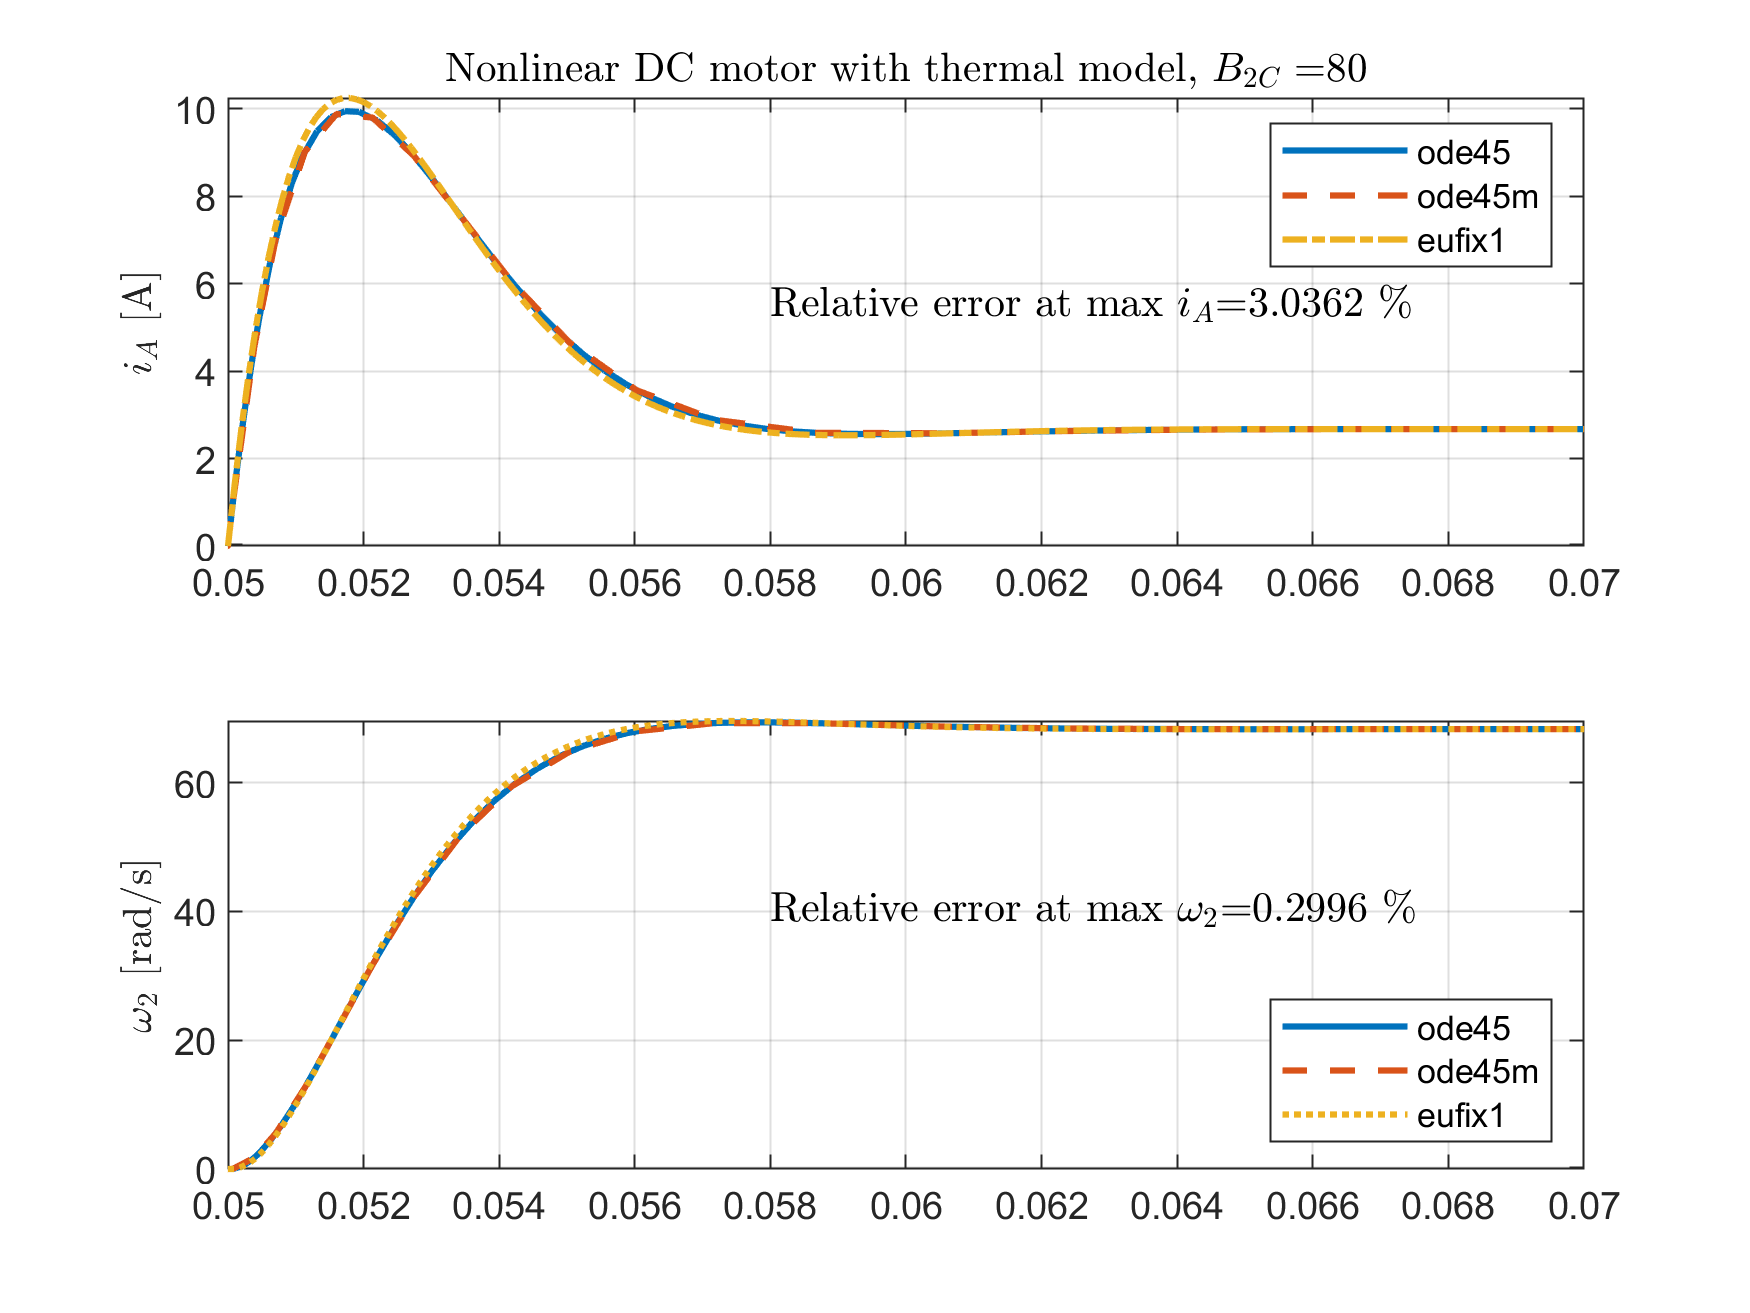
\includegraphics[width=0.80\linewidth]{E0_ode45-ode45m-eufix1_1e-4_zoom}
	\caption{Scenario 1: step size $1\times 10^{-4}$}
	\label{fig:Sce1_zoom_b}
\end{figure}

\subsection*{Scenario 2}
In this scenario we submitted the DC motor to high stiction $B_{2C}=300$ and sinsusoidal input at $5[Hz]$ which simulates the reversing mode. \tabref{tab:Sce2} shows the output for the three solvers showing that \texttt{ode45} is the slowest by far.

\begin{table}[!ht]
	\centering
	\scalebox{1}{
		\begin{tabular}{c|c|c|c}
			                     &  \bf{ode45}  & \bf{ode45m} & \bf{eufix1} \\
			\hline
			  simulation time [s]   & $517.798$ & $3.463$  & $0.093$  \\
			\hline
			number of time steps &  $13559913$  &   $9647$    &   $3002$
		\end{tabular} 		
	}
	\caption{Scenario 2: simulation time and number of steps.}
	\label{tab:Sce2}
\end{table}

\figref{fig:Sce2} shows the simulation output. The relevant result is the behavior of the system around the (nonlinear) stiction. $\omega_2$ sticks at $0.15[s]$ and $0.25[s]$ due to $B_{2C}$. 

\begin{figure}[H]
	\centering
	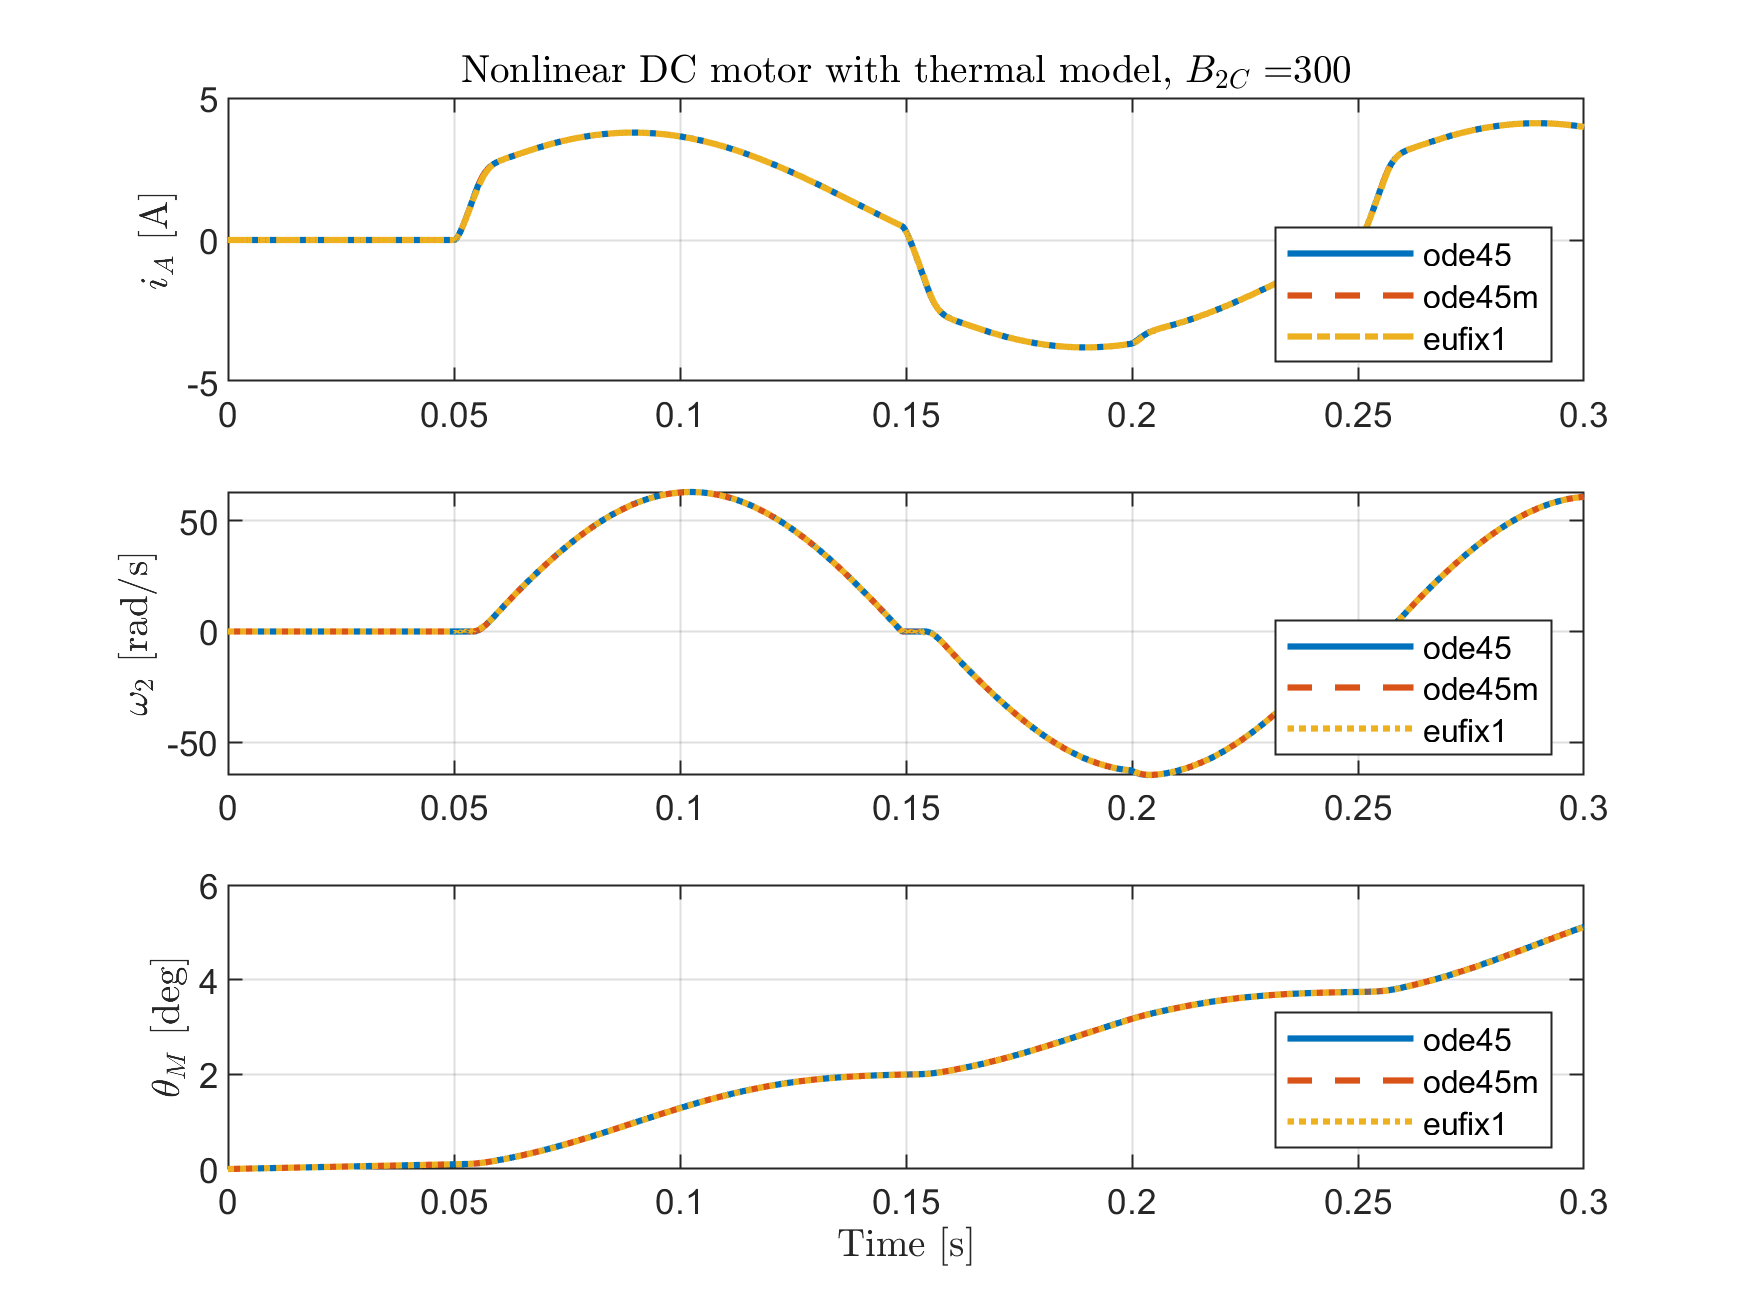
\includegraphics[width=0.8\linewidth]{sinE0_ode45-ode45m-eufix1_1e-4}
	\caption{Scenario 2: reversing mode.}
	\label{fig:Sce2}
\end{figure}

Even though the solvers were able to solve the dynamics with stiction, \texttt{ode45} took too much time to overcome this nonlinearity. \figref{fig:Sce2_zoom} shows the stiction with three different zoom levels for each solver. The fastest but with more integration step error is \texttt{eufix1}. \texttt{ode45m} has less error $\pm 0.01$, and finally \texttt{ode45} solves with the minimum error, around $\pm 10\times 10^{-5}$. In conclusion, \texttt{ode45m} is the best choice against the rest because it can obtain the solution with low error and with decent speed.

\begin{figure}[H]
	\centering
	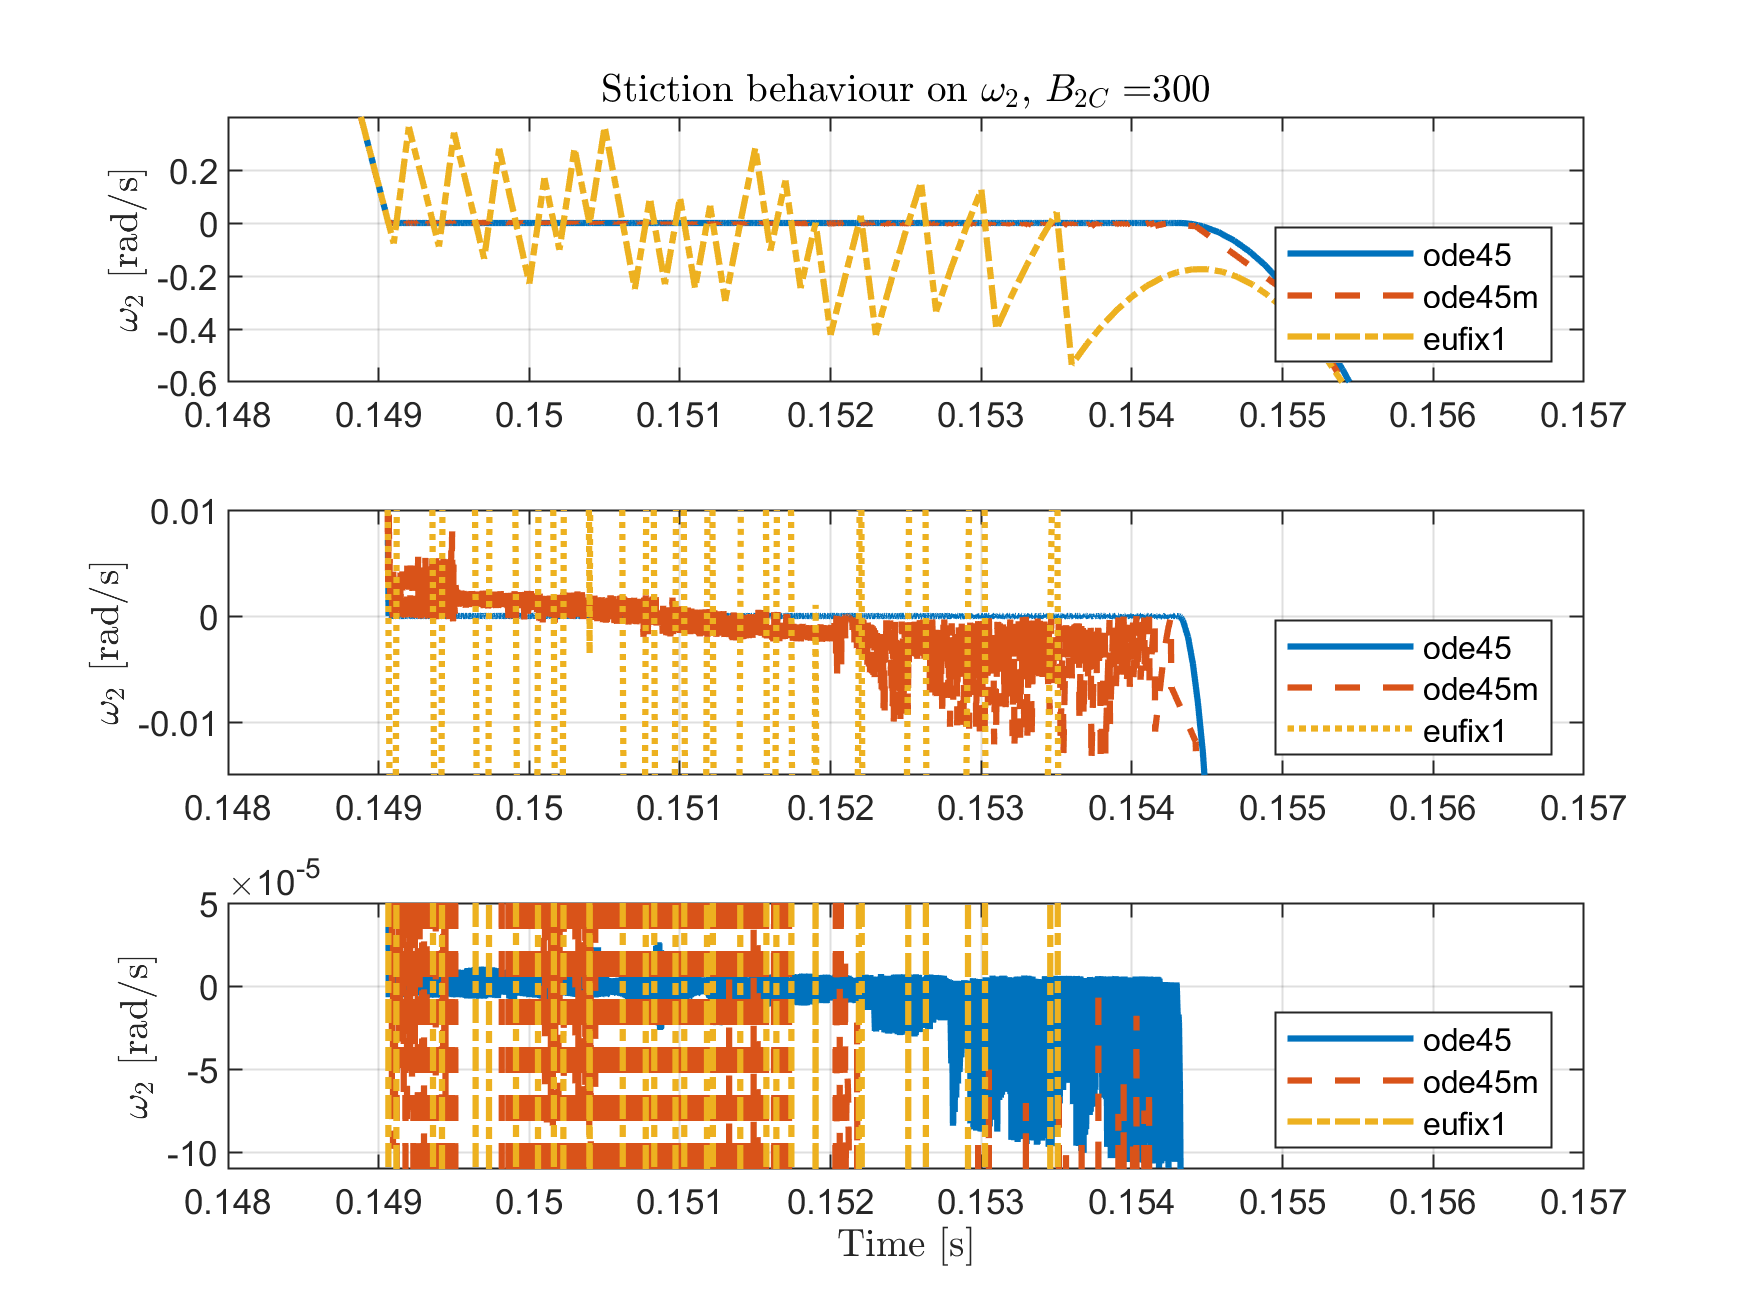
\includegraphics[width=1\linewidth]{sinE0_ode45-ode45m-eufix1_1e-4_zoom}
	\caption{Scenario 2: stiction behavior at $0.148\leq t \leq 0.157$.}
	\label{fig:Sce2_zoom}
\end{figure}

The motor temperature $\theta_M$ in reversing mode reaches the steady-state at $45[s]$ approximately which indicates the motor won't suffer overheat due to stiction. 
\begin{figure}[H]
	\centering
	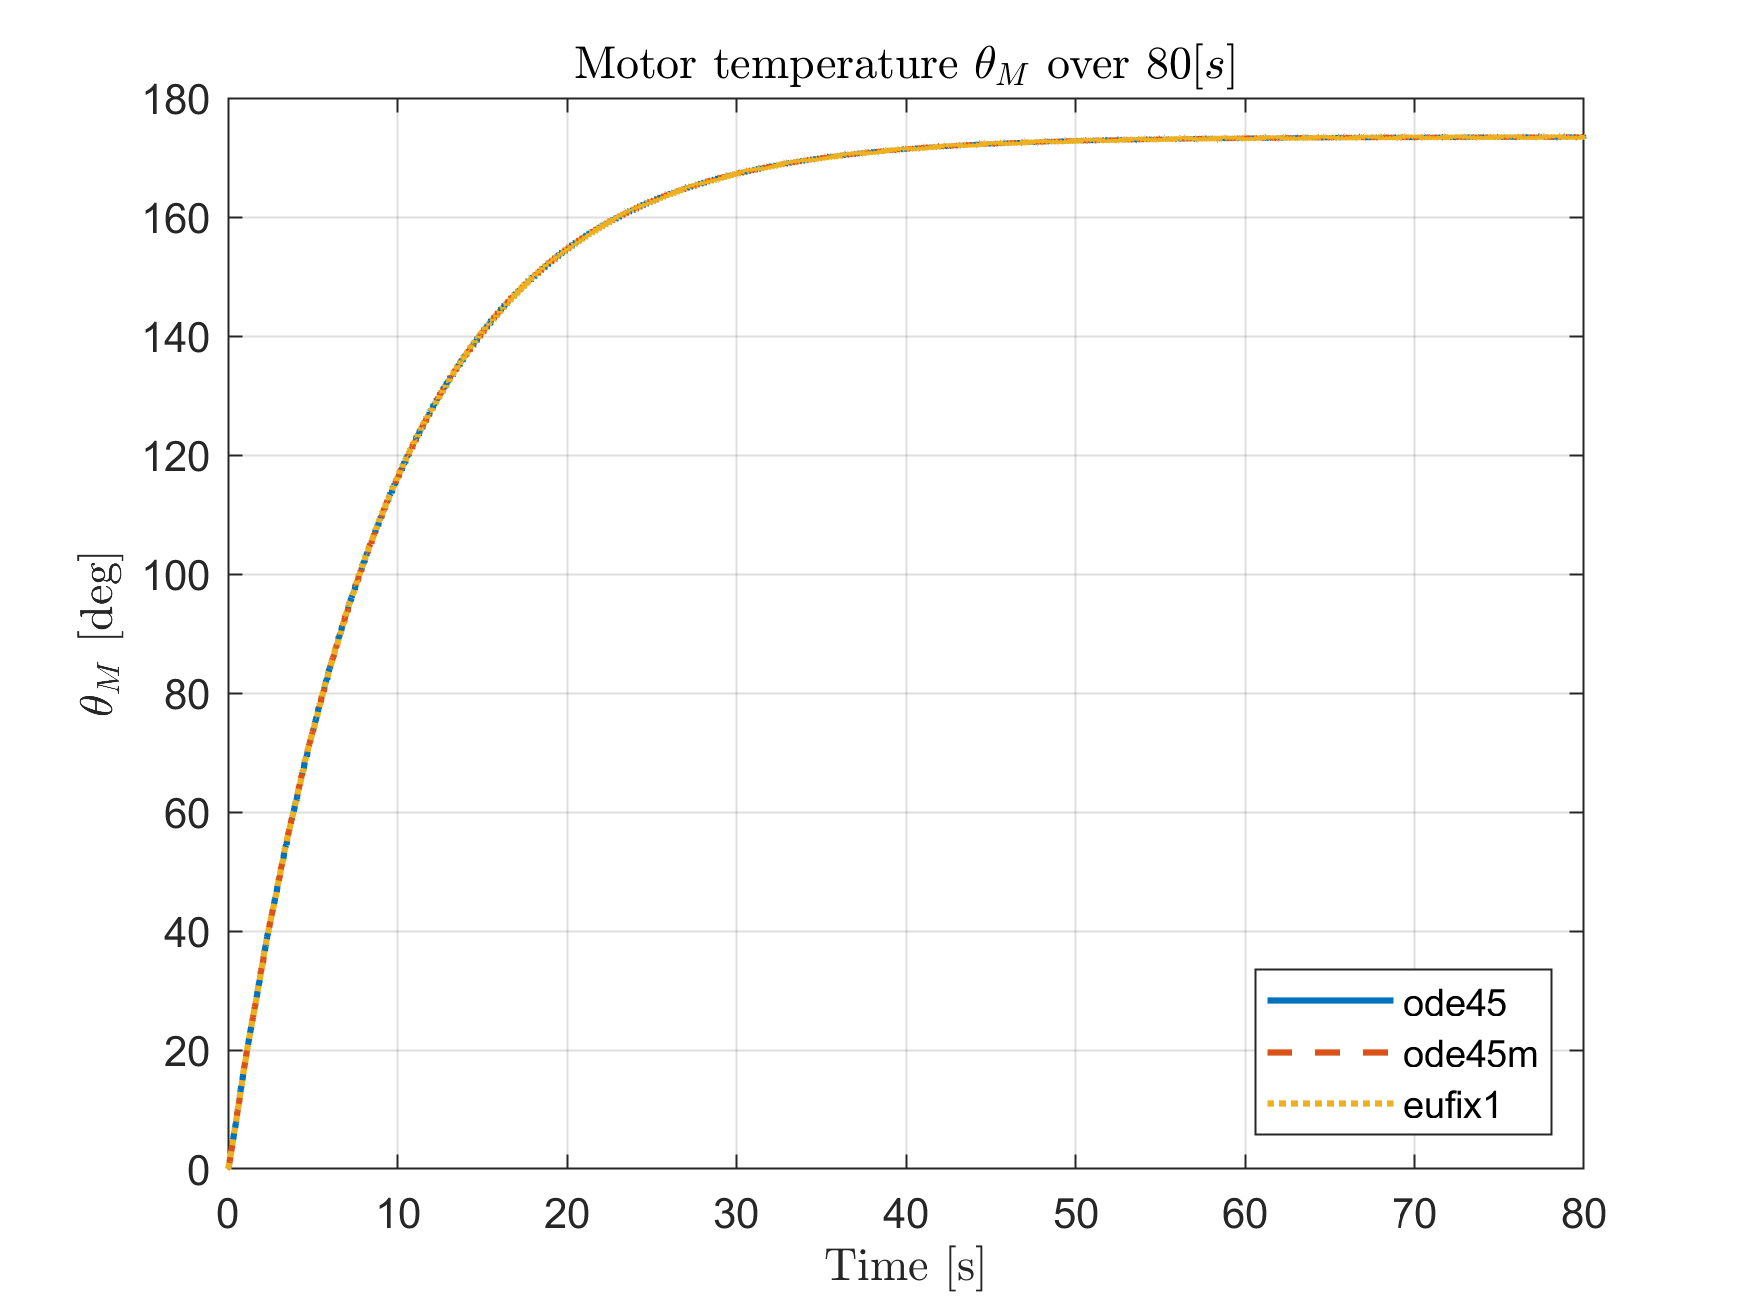
\includegraphics[width=0.65\linewidth]{sinE0_thetaM_ode45-ode45m-eufix1_1e-4}
	\caption{Scenario 2: motor temperature.}
	\label{fig:Sce2_stiction}
\end{figure}






\end{document}
